%!TEX root=main.tex

\section{Attack Analysis} \label{analysis}

Pasithea is intended to help investigate multiple types of attacks.
In particular, we observed and analyzed a distributed denial of service (DDoS) flood and the attempted use of cross-site scripting (XSS) commands.
In a DDoS attack, an attacker floods a network or service with information or requests in an attempt to exhaust some finite system resource such as memory~\cite{DoS-Def}. 
The goal of a DDoS attack varies, but it is most commonly intended to disrupt legitimate users from accessing information or services provided by the network.

The DDoS attack on G-star lasted from May 25, 2017 until June 1, 2017, creating over 275,000,000 log entries. 
During this time, the requests per second ($R/s$) steadily rose, starting at $500 R/s$ and peaking at over $6000 R/s$. 
As an unintended side effect, the log file grew to over 18 GB in size until G-star ran out of storage on its 20 GB cloud-hosted server.
The requests received during the DDoS attack all contained the command type $HEAD$ and the command text ``home''.

\begin{figure}[b]
   \centering
   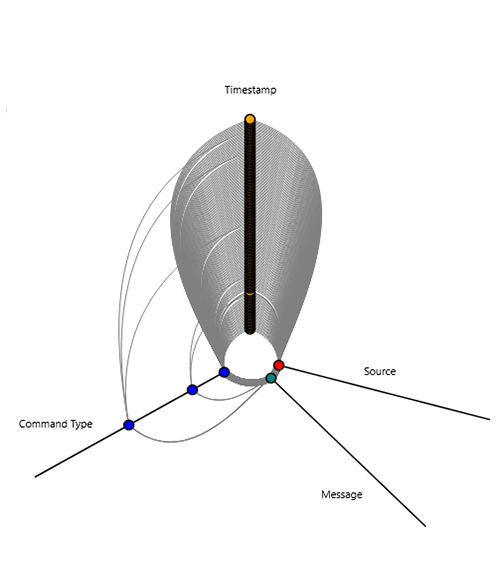
\includegraphics[width=2.5in]{images/regHive.png} 
   \caption{Hive plot displaying a random sample of 150 points from G-star logs. Data sampled is from February 6, 2017 -- May 25, 2017.}
   \label{fig:regHive}
\end{figure}

%% When citing figures in text IEEE wants them to be referenced as 'Fig. x' rather than Figure x
%% Okay.
We gathered a simple random sample of 150 requests collected by the G-star logs between February 6, 2017 and May 25, 2017 (a period covering normal operations and the attack).
This data was then rendered into a Hive plot~\cite{Hive-Plot} to interpret the attack. 
Hive plots are a perceptually uniform, scalable visualization for network analytics.  
We used a four-axis graph to reflect the relationships among timestamp, data source, command type, and response message (Fig.~\ref{fig:regHive}). 
The timestamp axis is the most heavily populated, containing distinct plotted points for each second during which a log entry was created. 
The source and message axes are closely related because there is only one plotted point on each axis. 
Source is the source of the response message returned by G-Star, and message is the response itself. 
In the context of the log file we analyzed, the source is always ``back-end'' (meaning the web server in this case) and message is always ``Unknown command:''. 
Lastly, the plotted points on the command type axis delineate unique HTTP request methods such as GET, POST, HEAD, PUT, DELETE, etc.

Fig.~\ref{fig:regHive} displays all 150 requests, while Fig.~\ref{fig:uniqHive} highlights the outlying requests that did not use the command type GET.  
Rather, these requests used the command types POST and HEAD. 
The POST requests are shown as the plotted point second closest to the center of the axis, while the HEAD requests are the farthest plotted point from the center of the axis. 
Fig.~\ref{fig:uniqHive} represents requests that used methods not commonly employed by web browsers or web crawlers, two of the most frequent sources of unwanted requests found in data gathered by Pasithea. 
This suggests these requests were deliberate and potentially malicious in nature.

\begin{figure}[t]
   \centering
   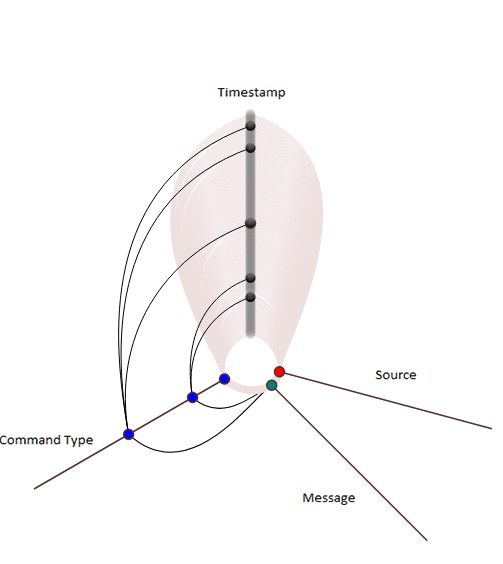
\includegraphics[width=2.5in]{images/uniqHive.png} 
   \caption{Prominent nodes denote ``injections'' into G-star that differ from normal traffic. Data sampled is from February 6, 2017 -- May 25, 2017}
   \label{fig:uniqHive}
\end{figure}

Cross-site scripting attacks aim to inject malicious scripts into an otherwise benign or trusted website~\cite{XSS-def}. 
Further investigation of the specific commands being attempted as an XSS attack revealed the following:

\noindent \texttt{GET cgi\\     
POST command.php\\
GET ;rm\$IFS-f\$IFS’'\\
GET ;wget\$IFS-O\$IFS’'\\
GET ;chmod\$IFS'’777’'\$IFS’'\\
GET ;sh\$IFS-c\$IFS‘'}

\noindent Fig. \ref{fig:XSS} displays a selected sample of entries collected by the G-star logs between March 11, 2017 and March 16, 2017. 
The highlighted requests have a span of 25 seconds where the XSS commands were attempted.
This shows both the short amount of time it took to run this malware insertion attempt and the use of GET and POST request methods for one attack.

We determined that a very similar attack sequence was also recently documented by a Finnish cyber-security company F-Secure~\cite{F-Secure}. 
The commands attempted with the XSS attack are intended to upload a PHP: Hypertext Preprocessor (PHP) file, then send a series of commands that, if executed, would remove a file using the \$IFS variable found in PHP. 
Afterwards, it would attempt to download a file with the same variable name and change the permissions on said file so that it can be executed by any user.  
Then the attacker would execute the file. 
Researchers from F-Secure  attribute this attack profile to a Peer to Peer (P2P) botnet named TheMoon~\cite{TheMoon}. 
This example illustrates how we can use data collected from attack attempts to isolate and attribute the attack, provided that we can determine what types of attacks are taking place.

%% Q: How do we get this to appear in the right column like earlier?
%% A: Move it lower in the text. 
\begin{figure}[t]
   \centering
   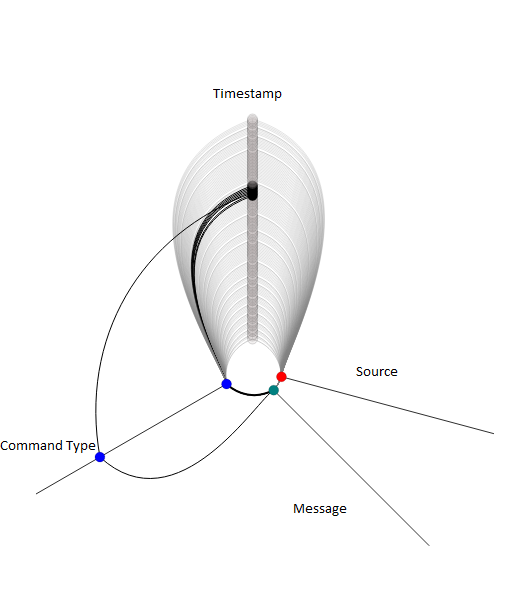
\includegraphics[width=2.5in]{images/XSS.png}  
   \caption{Prominent nodes display the XSS attempt on G-star. Data sampled is from March 11, 2017 -- March 16, 2017}
   \label{fig:XSS}
\end{figure}

Pasithea was subsequently deployed and is currently active on our AWS EC2 instance in Ashburn, Virginia. 
Our log files indicate cursory web crawls from Baidu, a Chinese search engine, and some attempts at exploiting a known vulnerability in Apache Tomcat web servers using ``GET /manager/html''~\cite{Tomcat-Exploit}. 
We continue to monitor this instance and additional results will be reported in future papers.
